% CAp 2026 submission — compile: pdflatex main && bibtex main && pdflatex main && pdflatex main
\PassOptionsToPackage{english}{babel}
\documentclass{pfia}

% Packages not loaded by pfia.cls
\usepackage{amsmath, amssymb}
\usepackage{booktabs}
\usepackage{graphicx}
\usepackage{algorithm}
\usepackage{algpseudocode}
\usepackage{natbib}
\usepackage{xcolor}

% Colors required by pfia.cls hypersetup
\definecolor{afiablue}{RGB}{61,159,207}
\definecolor{afiared}{RGB}{167,75,68}
\definecolor{afialightblue}{RGB}{158,193,232}

\bibliographystyle{plainnat}

% ------------------------------------------
\title{\textbf{Opportunistic Targeting: Early Directional Commitment for\\Query-Efficient Black-Box Adversarial Attacks}}

% TODO: fill in affiliation and email before submission
\author{Florent Tariolle\fup{1} \\[6pt]
\fup{1} TODO: Affiliation}

\date{TODO: email}

\begin{document}

\maketitle

% ------------------------------------------
\begin{resume}
Les attaques adversariales en boîte noire qui minimisent uniquement la confiance de la classe correcte souffrent de \textit{dérive de classe}: les perturbations explorent l'espace des caractéristiques sans s'engager vers une classe cible, gaspillant des requêtes. Nous proposons l'\textbf{Opportunistic Targeting} (OT), un wrapper qui bascule une attaque non ciblée vers un objectif ciblé tôt dans sa trajectoire, se verrouillant sur la classe non vraie dominante. Validé sur SimBA, Square Attack et Bandits avec cinq classifieurs ImageNet (4\,500 exécutions), OT atteint des performances proches de l'oracle sur les attaques par recherche aléatoire (+27 points sur ResNet-50 pour SimBA), mais n'apporte rien aux attaques par estimation de gradient, confirmant son rôle de surrogate de marge. Sur les modèles entraînés de manière adversariale, l'effet est neutre. Le bénéfice provient de l'engagement directionnel précoce, indépendamment du mécanisme de déclenchement.
\end{resume}

\begin{motscles}
Attaques adversariales, boîte noire, efficacité en requêtes, ciblage opportuniste.
\end{motscles}

\begin{abstract}
Black-box adversarial attacks that minimize only the ground-truth confidence suffer from \textit{class drift}: perturbations wander through the feature space without committing to a specific adversarial class, wasting queries on diffuse, undirected progress. We introduce \textbf{Opportunistic Targeting (OT)}, a lightweight wrapper that switches an untargeted attack to a targeted objective early in its trajectory, locking onto whichever non-true class currently leads. OT requires no architectural modification to the underlying attack, no gradient access, and no \textit{a priori} target-class knowledge.

We validate OT on three score-based attacks---SimBA, Square Attack (cross-entropy loss), and Bandits---across five standard ImageNet classifiers including a Vision Transformer (4,500 runs). On random-search attacks, OT closely tracks oracle performance: SimBA success rate rises from 43\% to 70\% on ResNet-50 (+27 pp), and Square Attack achieves a 43\% censored-mean iteration reduction. On the gradient-estimation attack Bandits, OT provides no benefit---a negative result that reinforces our margin-surrogate interpretation. On adversarially-trained models, targeting mode has no statistically significant effect. The benefit is driven by early directional commitment itself: a fixed-iteration switch performs identically to a rank-stability heuristic across all tested configurations.
\end{abstract}

\begin{keywords}
Adversarial attacks, black-box, query efficiency, opportunistic targeting.
\end{keywords}

% ============================================================================
\section{Introduction}\label{sec:introduction}

Standard untargeted black-box attacks minimize the model's confidence in the ground-truth class. This strategy, whether implemented as probability minimization in SimBA \citep{guo2019simple} or cross-entropy loss in Square Attack \citep{andriushchenko2020square}, treats all non-true classes as interchangeable. The freed probability mass spreads across remaining classes without directional commitment---the perturbation executes a random walk through the latent space, crossing class basins opportunistically rather than heading toward a specific decision boundary.

This \textit{class drift} directly impacts query efficiency. Each query spent exploring a class basin that will ultimately be abandoned is wasted. The deeper the model, the more basins the perturbation traverses before settling, and the more pronounced the waste becomes.

Targeted attacks eliminate drift by construction but require specifying a target class \textit{a priori}, which is generally unavailable in a black-box setting. Margin-based losses \citep{carlini2017towards} offer a partial solution by implicitly tracking the nearest decision boundary, but not all attacks support them. SimBA operates on raw probabilities; other attacks use cross-entropy for compatibility. For these methods, drift remains the main efficiency bottleneck.

\textbf{Opportunistic Targeting} bridges this gap with a two-phase strategy:
\begin{enumerate}
    \item \textbf{Exploration phase.} The attack runs in untargeted mode for a short prefix of $T$ iterations.
    \item \textbf{Exploitation phase.} The attack switches to a targeted objective against the leading non-true class, and runs until misclassification or budget exhaustion.
\end{enumerate}

The switch timing $T$ is not sensitive: ablations show that any $T \in \{5, \ldots, 500\}$ yields statistically indistinguishable results (Section~\ref{sec:naive-ablation}), because class rankings stabilize within the first few iterations for drift-prone attacks. This paper makes three contributions:

\begin{enumerate}
    \item \textbf{A wrapper for drift-prone score-based attacks} that adds opportunistic targeting. OT benefits random-search attacks (SimBA, Square Attack with CE loss) but not attacks with built-in directionality (gradient estimation, margin loss), confirming its role as a margin surrogate.
    \item \textbf{Empirical validation} across five ImageNet classifiers and three attack methods (4,500 runs), showing that OT provides near-oracle efficiency. The benefit is driven by early directional commitment: a fixed-iteration switch performs identically to a rank-stability heuristic.
    \item \textbf{A characterization of targeting neutrality} on adversarially-trained models, where a bimodal difficulty distribution eliminates the medium-difficulty regime where directional commitment provides value.
\end{enumerate}

Beyond the practical wrapper, our results reveal a structural property of untargeted adversarial loss landscapes: the information needed to select an effective target is already latent in the attack's trajectory after just a few iterations.

% ============================================================================
\section{Related Work}\label{sec:related-work}

\subsection{Score-Based Black-Box Attacks}\label{sec:score-based}

Score-based attacks assume access to the full output probability vector but not to gradients. SimBA \citep{guo2019simple} iterates over an orthonormal basis (pixel or DCT), accepting perturbations that reduce the true-class probability (1.4--1.5 queries per iteration on average). Its original formulation provides no mechanism for directing perturbations toward a specific adversarial class.

Square Attack \citep{andriushchenko2020square} uses random square-shaped patches at the vertices of the $L_\infty$ ball, with a schedule that shrinks the patch size as the attack progresses. Its default margin loss $f_{y}(x) - \max_{k \neq y} f_k(x)$ implicitly tracks the nearest decision boundary. When run with cross-entropy loss, this guidance vanishes and the attack exhibits drift, making it an ideal testbed for isolating OT's contribution.

\subsection{Gradient-Estimation Attacks}\label{sec:gradient-estimation}

ZOO \citep{chen2017zoo} uses coordinate-wise finite differences; Bandits \citep{ilyas2019prior} accelerates convergence by incorporating data-dependent priors into the gradient estimate. Unlike random-search attacks, gradient-estimation attacks have built-in directionality analogous to margin loss. SignHunter \citep{aldujaili2020sign} further simplifies this by estimating only the sign of the gradient. We test OT on Bandits in Section~\ref{sec:results} to determine whether the wrapper provides value when the underlying attack already has directional information.

\subsection{Decision-Based Attacks and Angular Convergence}\label{sec:decision-based}

Decision-based attacks require only the top-1 label. SurFree \citep{maho2021surfree} uses random 2-D hyperplane search, and \citet{gesny2024gradient} show that reintroducing gradient estimation (yielding CGBA) accelerates convergence of the angle $\theta(i)$ between the current perturbation direction and the optimal adversarial direction. This is loosely analogous to OT: both methods reintroduce directional information into a blind search process. We adopt the same angular convergence framework in Section~\ref{sec:theta-convergence}.

Adversarially-trained models \citep{madry2018towards,salman2020adversarially}, standardized via RobustBench \citep{croce2021robustbench}, present a qualitatively different challenge with flatter loss landscapes and more uniform confidence distributions. Section~\ref{sec:robust} examines whether OT remains useful in this regime.

% ============================================================================
\section{Method}\label{sec:method}

\subsection{Notation}\label{sec:notation}

Let $f: \mathcal{X} \to \mathbb{R}^K$ denote a classifier mapping inputs to logits over $K$ classes, and $P(k|x) = \text{softmax}(f(x))_k$ the predicted probability of class $k$. Given a correctly-classified input $x$ with true label $y$, the attacker seeks an adversarial example $x' = x + \delta$ such that $\arg\max_k P(k|x') \neq y$ and $\|\delta\|_\infty \leq \epsilon$.

\subsection{Untargeted Loss and the Drift Problem}\label{sec:drift}

Standard untargeted attacks minimize a loss that depends only on the true class:
\begin{equation}
\mathcal{L}_{\text{untarg.}}(x', y) = P(y | x') \;\text{(SimBA)} \quad \text{or} \quad -\log P(y | x') \;\text{(CE)}
\end{equation}
These objectives decrease $P(y|x')$ without specifying where the freed probability mass should concentrate. We call this \textit{class drift}. \textbf{Margin loss} avoids drift by construction:
\begin{equation}
\mathcal{L}_{\text{margin}}(x', y) = f_y(x') - \max_{k \neq y} f_k(x')
\end{equation}
where $\max_{k \neq y} f_k(x')$ dynamically identifies the nearest competitor. Square Attack's default loss is of this form, explaining its strong untargeted performance.

A targeted attack toward class $t$ optimizes $\mathcal{L}_{\text{targeted}}(x', t) = -P(t | x')$ (SimBA) or $\log P(t | x')$ (CE). Targeting eliminates drift but requires knowing $t$ in advance. An \textit{oracle} target---the class the unconstrained untargeted attack eventually reaches---provides a trajectory-specific performance ceiling that no real attacker can achieve.

\subsection{Opportunistic Targeting Algorithm}\label{sec:algorithm}

OT discovers the target class online by observing which adversarial class the perturbation is naturally drifting toward.

\textbf{Fixed-iteration switch (recommended).} The attack runs in untargeted mode for $T$ iterations, then switches to a targeted objective against $t = \arg\max_{k \neq y} P(k|x')$. Ablations (Section~\ref{sec:naive-ablation}) show that $T \in \{5, \ldots, 500\}$ all yield indistinguishable results, so any small $T$ suffices.

\textbf{Rank-stability variant.} A stability counter tracks the leading non-true class after each accepted perturbation step, switching only after the same class leads for $S$ consecutive accepted steps (Algorithm~\ref{alg:ot}). In practice, this provides no measurable advantage over the fixed switch (Section~\ref{sec:naive-ablation}). We retain it for completeness.

\begin{algorithm}[t]
\caption{Opportunistic Targeting (Rank-Stability Variant)}
\label{alg:ot}
\begin{algorithmic}[1]
\Require image $x$, true label $y$, attack $A$, stability threshold $S$
\Ensure adversarial example $x'$
\State $x' \leftarrow x$, $\textit{locked} \leftarrow \text{False}$, $\textit{target} \leftarrow \text{None}$, $\textit{candidate} \leftarrow \text{None}$, $\textit{streak} \leftarrow 0$
\While{not misclassified($x'$) and budget not exhausted}
    \State $\textit{mode} \leftarrow \text{targeted if } \textit{locked} \text{ else untargeted}$
    \State $x' \leftarrow A.\text{step}(x', y \text{ if not } \textit{locked} \text{ else } \textit{target}, \textit{mode})$
    \If{step was accepted}
        \State $c \leftarrow \arg\max_{k \neq y} P(k | x')$
        \If{not \textit{locked}}
            \If{$c = \textit{candidate}$} $\textit{streak} \leftarrow \textit{streak} + 1$
            \Else{} $\textit{candidate} \leftarrow c$; $\textit{streak} \leftarrow 1$
            \EndIf
            \If{$\textit{streak} = S$} $\textit{target} \leftarrow \textit{candidate}$; $\textit{locked} \leftarrow \text{True}$
            \EndIf
        \EndIf
    \EndIf
\EndWhile
\State \Return $x'$
\end{algorithmic}
\end{algorithm}

Once a target is locked, the attack commits for the remainder of the budget (\textbf{irreversible lock}). Releasing the lock would re-introduce the exploration overhead that OT is designed to eliminate.

\subsection{Attack Integration}\label{sec:integration}

\textbf{SimBA.} We use the DCT basis with $8\times8$ blocks, $\epsilon = 8/255$ in $L_\infty$, and a 10,000-query budget. In untargeted mode, SimBA reduces $P(y|x')$; upon lock-in, the criterion switches to increasing $P(t|x')$. The perturbation mechanism is unchanged.

\textbf{Square Attack (CE loss).} We deliberately run Square Attack with cross-entropy loss rather than its default margin loss. This is a methodological choice to isolate OT's contribution: margin loss already provides implicit target tracking (Section~\ref{sec:drift}), which would confound OT's effect. This choice demonstrates OT's \emph{mechanism}; practitioners using Square Attack should keep the default margin loss, which already provides the directionality that OT adds. Budget is $N = 10{,}000$ iterations; the patch schedule depends on $N$, so all experiments use a fixed $N$ for comparability.

\textbf{Bandits.} Bandits \citep{ilyas2019prior} estimates gradients with data-dependent priors, providing built-in directionality analogous to margin loss. We use the stability variant ($S = 15$), 5,000-iteration budget, $\epsilon = 8/255$.

% ============================================================================
\section{Experimental Setup}\label{sec:setup}

\textbf{Models.} We evaluate on five standard ImageNet classifiers from torchvision (AlexNet, ResNet-18, VGG-16, ResNet-50, ViT-B/16 \citep{dosovitskiy2021image}), wrapped with a \texttt{NormalizedModel} so all attacks operate in $[0, 1]$ pixel space. ViT-B/16 tests whether OT's benefit depends on convolutional inductive biases. We also evaluate two adversarially-trained models from RobustBench \citep{salman2020adversarially,croce2021robustbench}: Salman2020Do\_R18 and Salman2020Do\_R50.

\textbf{Protocol.} Each (model, attack, image) triplet is evaluated in three modes: \textit{untargeted} (standard attack), \textit{targeted oracle} (target class chosen \textit{a posteriori} from the untargeted result, providing a trajectory-specific ceiling), and \textit{opportunistic} (OT). The oracle is determined by running a probe untargeted attack with the same random seed; it is not globally optimal---a geometry-based target might yield shorter paths---but provides a reproducible reference for the perturbation path the attack would have followed.

\textbf{Configuration.} Perturbation budget $\epsilon = 8/255$ ($L_\infty$). Query budget: 10,000 iterations (main benchmark) and 15,000 (extended benchmark). Stability thresholds: $S = 10$ (SimBA), $S = 8$ (Square Attack) on standard models; $S = 10$ for both on robust models.

\textbf{Images.} 100 images randomly sampled from ILSVRC2012 validation (seed 42). Each combination uses a single attack random seed (seed 0), yielding 4,500 runs on standard models. We acknowledge the single seed as a limitation (Section~\ref{sec:limitations}).

\textbf{Metrics.} Primary: \textit{success rate} at equal query budgets. We also report \textit{success rate vs.\ query budget} (CDF curves) following \citet{ughi2021empirical}. Secondary: \textit{censored mean iterations} (failed runs capped at budget ceiling, capturing both efficiency and success-rate gains) and \textit{paired mean iterations} (restricted to images where both modes succeed, isolating pure efficiency). Censoring biases \emph{against} OT, making savings estimates conservative.

% ============================================================================
\section{Results on Standard Networks}\label{sec:results}

\subsection{Success Rates}\label{sec:success-rates}

Across 4,500 runs, OT closely tracks oracle-targeted success rates for random-search attacks. SimBA improves from 67\% untargeted to 75\% OT (oracle: 76\%), with the largest gain on ResNet-50: 43\% $\to$ 70\% (+27 pp). Square Attack (CE) improves from 96.2\% to 97.6\% (oracle: 99\%), with a pronounced effect on harder models (ResNet-50: 81\% $\to$ 94\%; ViT-B/16: 100\% with 16\% iteration savings).

Bandits shows no benefit from OT: success rates are flat or slightly negative across all models (e.g., VGG-16: 49\% $\to$ 41\%). Even oracle-targeted Bandits provides no improvement, confirming that gradient estimation already provides the directionality OT adds.

\begin{figure*}[t]
\centering
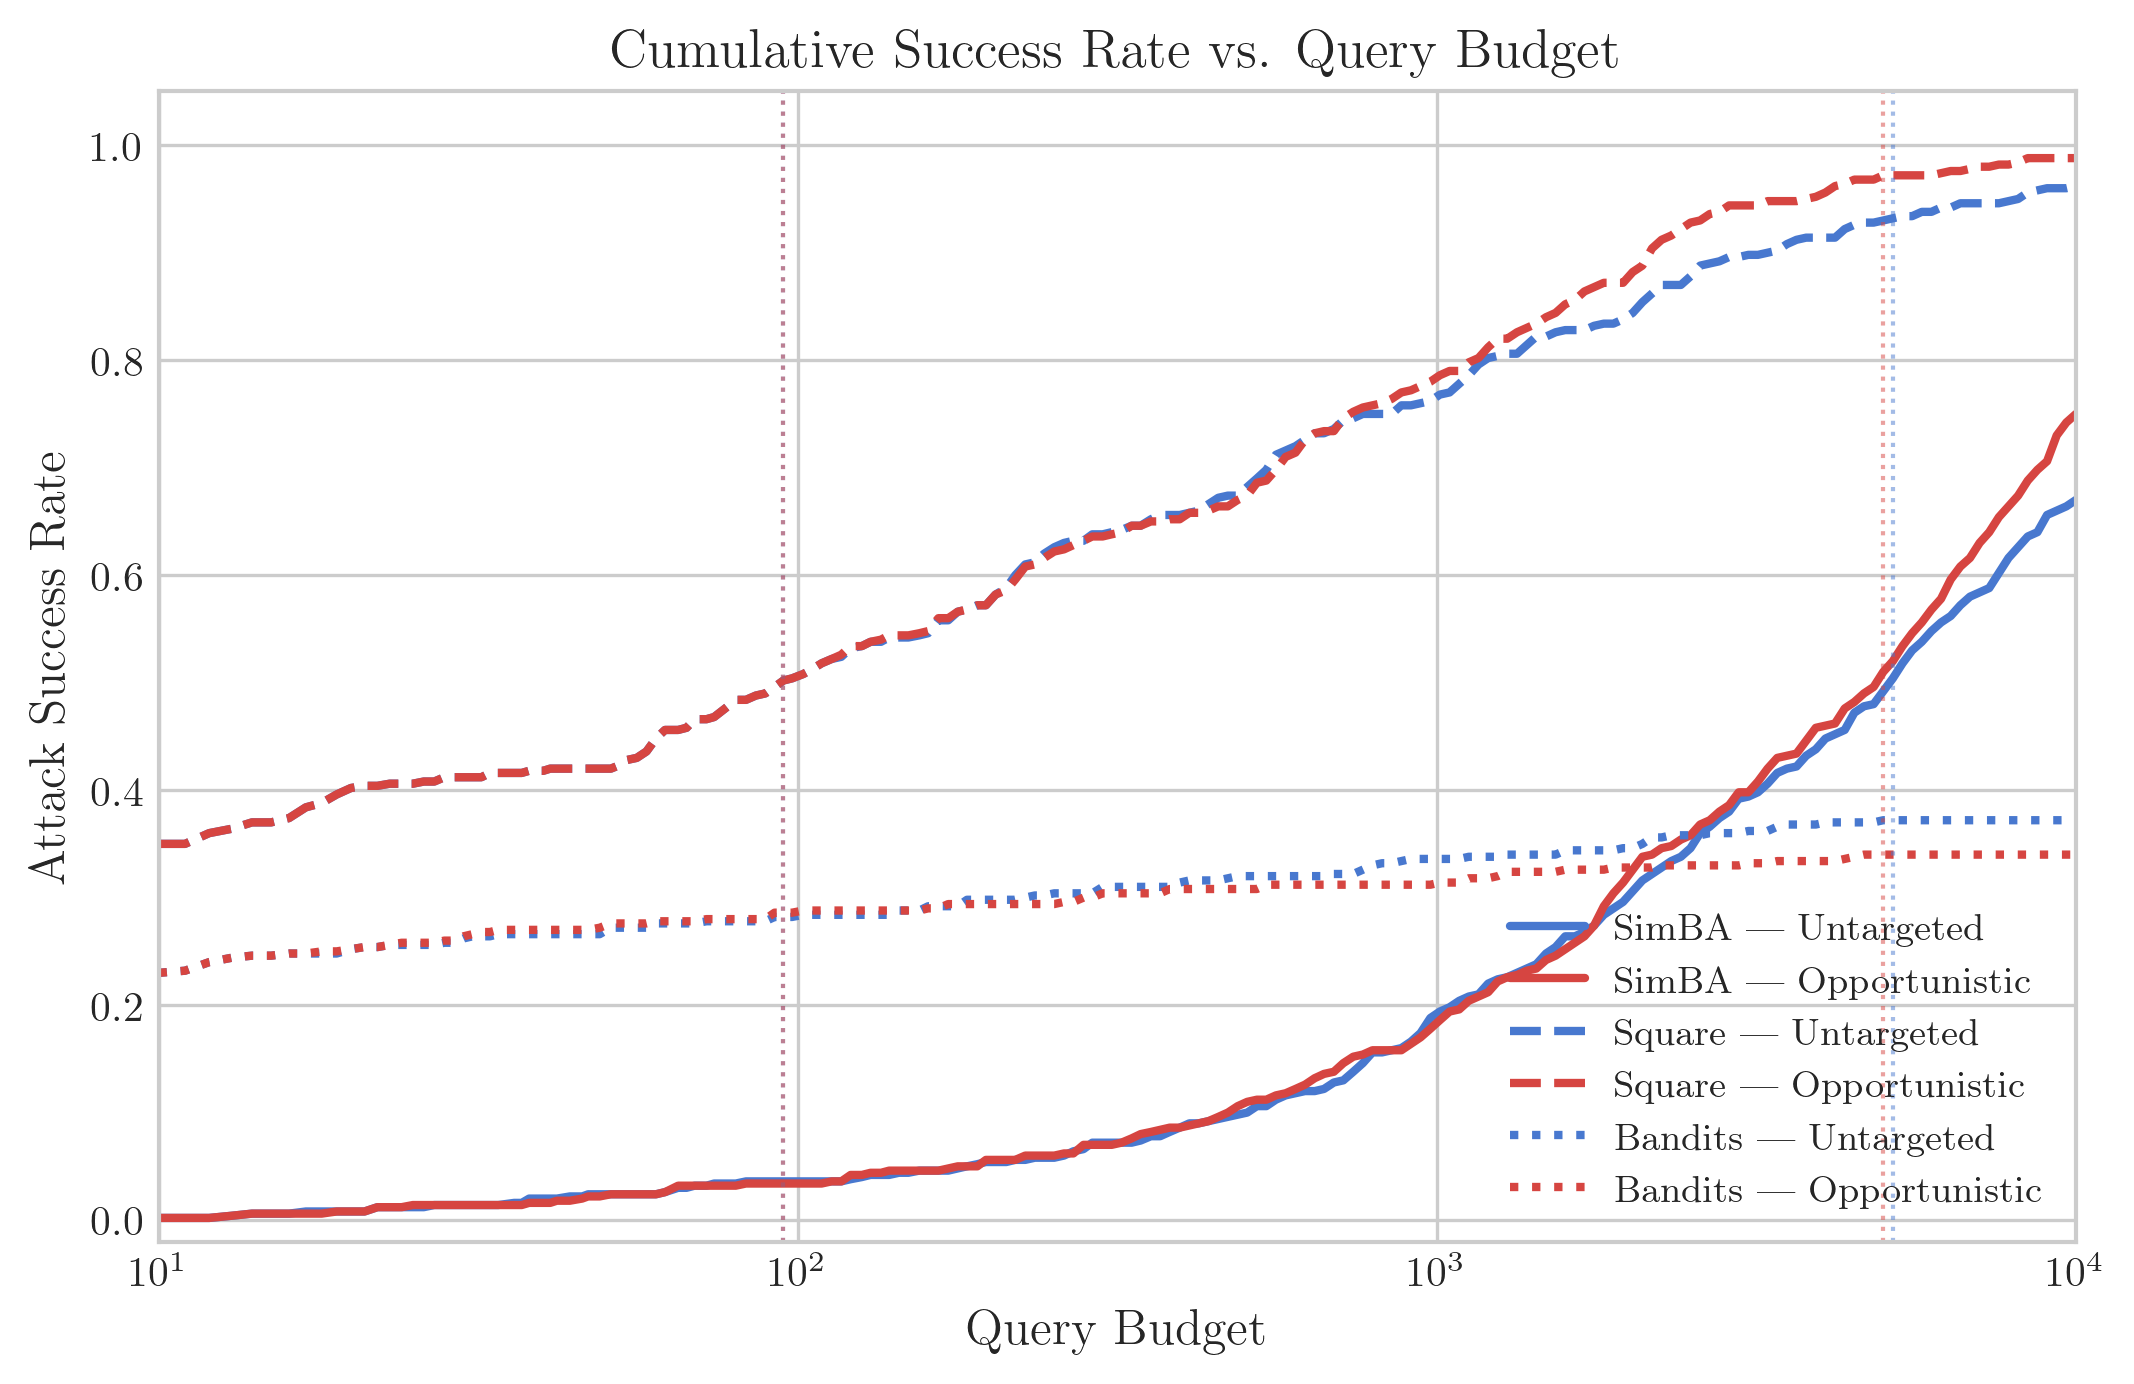
\includegraphics[width=0.85\textwidth]{../results/figures/standard/fig_cdf.png}
\caption{Success rate vs.\ query budget (100-image benchmark, all 5 standard models pooled). SimBA and Square Attack (CE) show clear OT benefit (green tracks oracle in orange). Bandits (dotted) shows no separation, confirming that gradient estimation already provides directionality.}
\label{fig:cdf-pooled}
\end{figure*}

\subsection{Iteration Efficiency}\label{sec:iteration-efficiency}

All Wilcoxon tests are two-sided signed-rank tests with Bonferroni correction across models.

\textbf{Censored mean} (failed = 10K ceiling). SimBA: OT reduces the censored mean by 4.8\% (5,426 $\to$ 5,164). Square Attack (CE): 29.5\% reduction (1,076 $\to$ 759). Bandits: slight increase of 3.7\% (3,254 $\to$ 3,374). SimBA and Square Attack show highly significant pooled Wilcoxon tests ($p < 10^{-9}$, Bonferroni-corrected). For Square Attack, per-model significance concentrates on ResNet-50 and ViT-B/16; easy models show floor effects ($<$100 iterations regardless of mode). For Bandits, no comparison reaches significance.

\begin{figure*}[t]
\centering
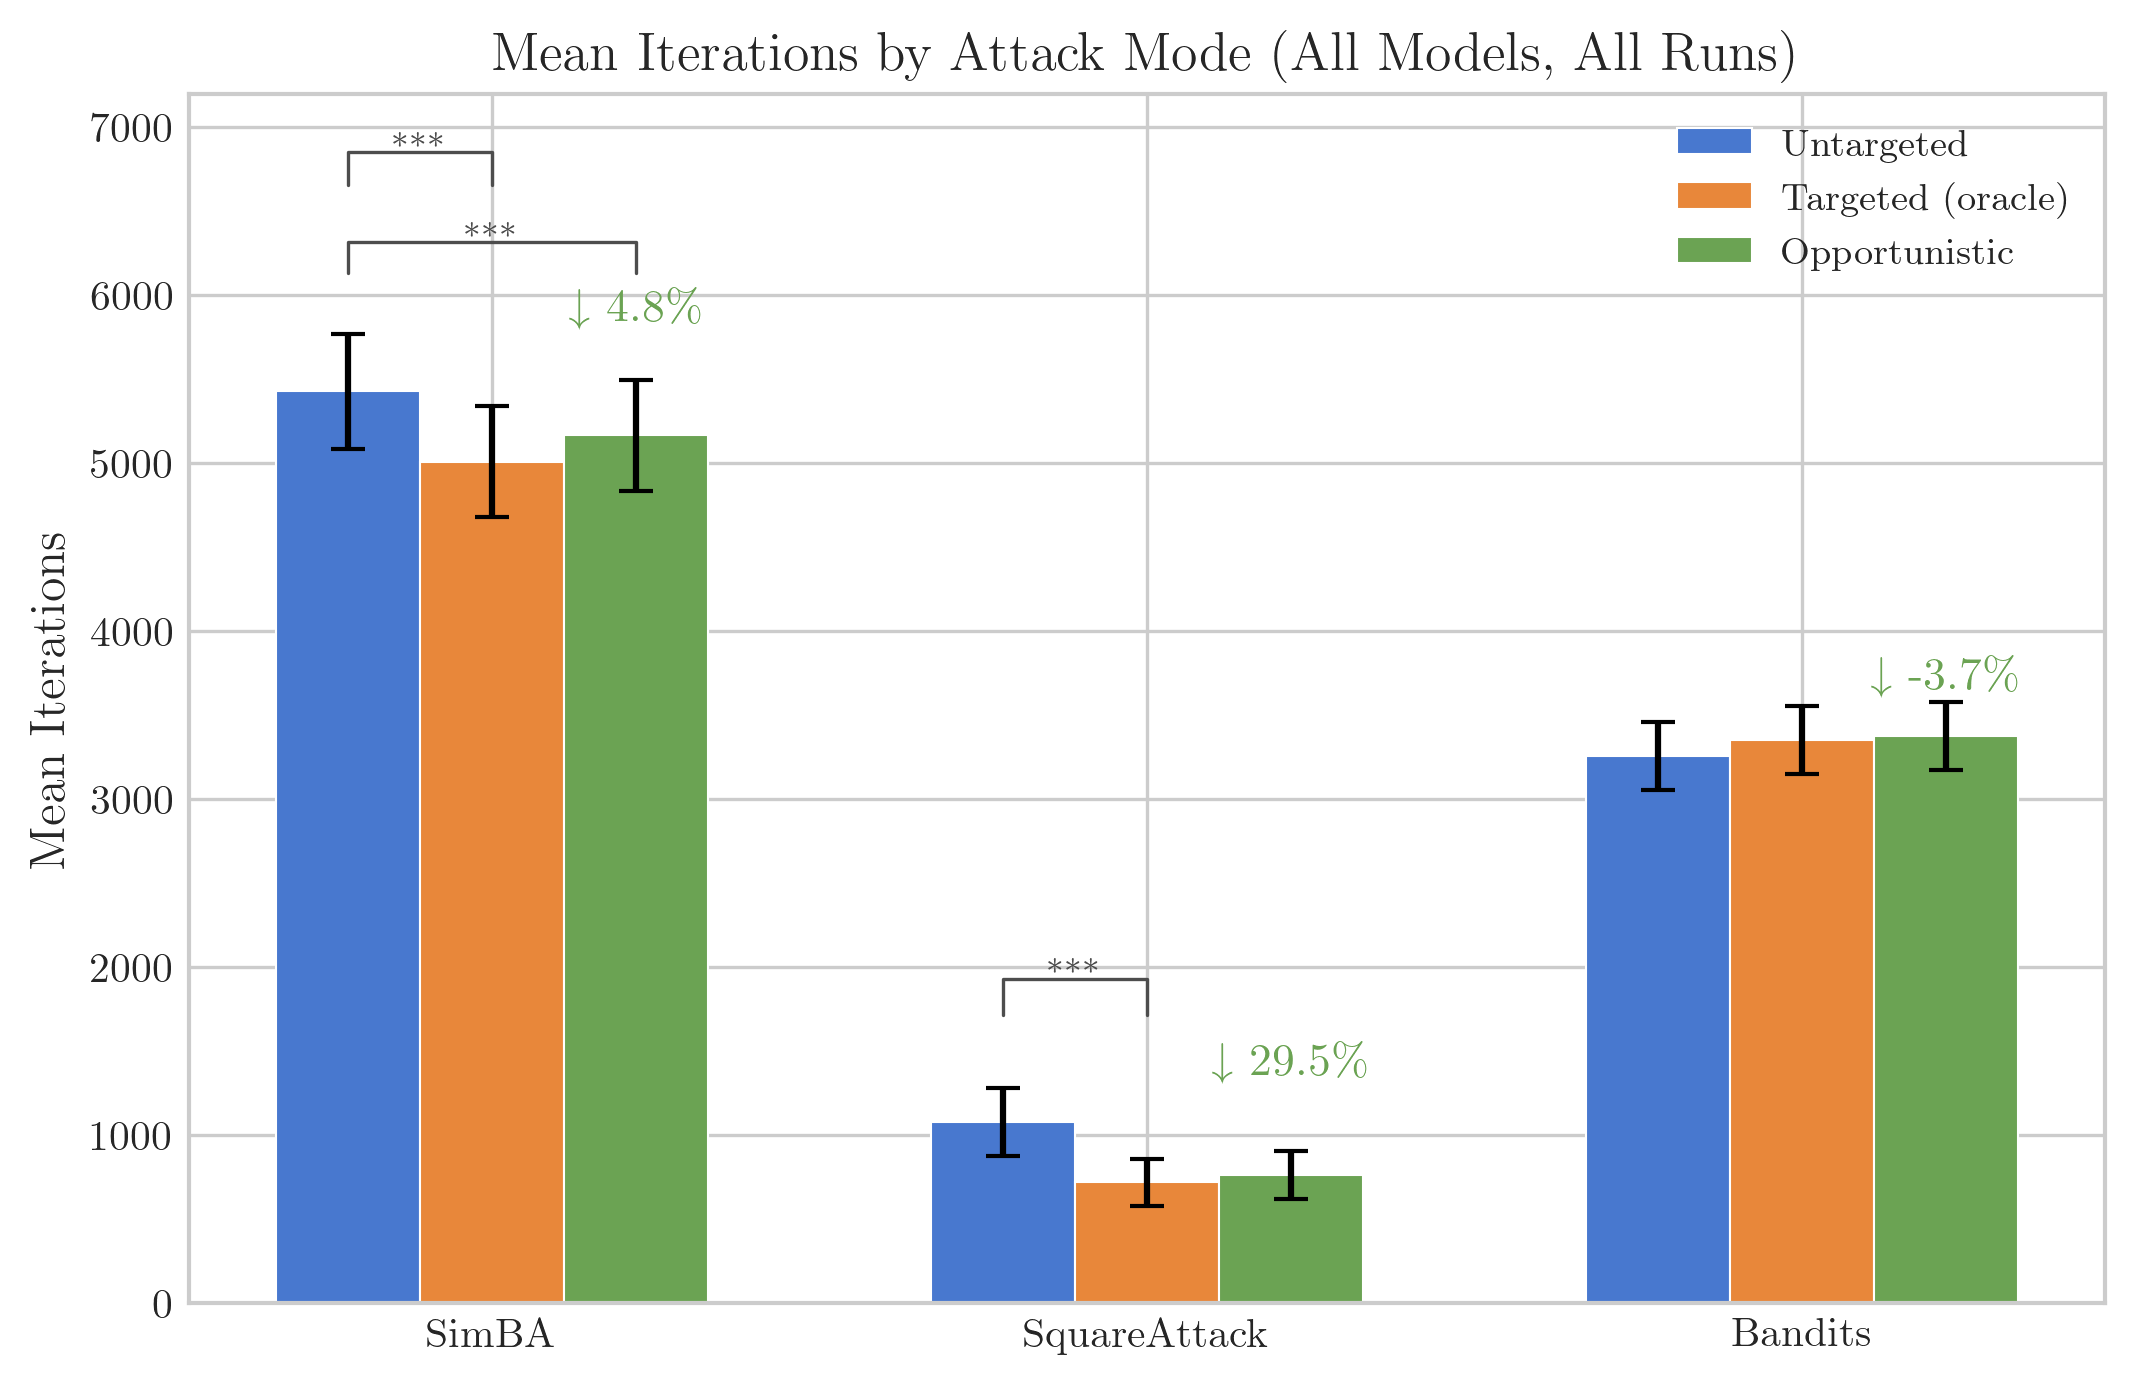
\includegraphics[width=0.85\textwidth]{../results/figures/standard/fig_headline_bars.png}
\caption{Censored mean iterations by attack mode (4,500 runs; failed runs assigned 10K ceiling). Error bars show 95\% bootstrap CI. Significance brackets show Bonferroni-corrected Wilcoxon signed-rank tests (pooled across models).}
\label{fig:headline-bars}
\end{figure*}

\subsection{Difficulty-Dependent Benefit}\label{sec:depth-scaling}

The largest gains appear on ResNet-50 and ViT-B/16---the two hardest models. We initially hypothesized this scaled with model depth, but the inclusion of ViT-B/16 (12 transformer blocks) and the anomalous behavior of VGG-16 (16 layers, negligible OT benefit) suggest that \textit{attack difficulty}---not depth per se---is the driver. The difficulty--savings scatter plot (Appendix~\ref{app:secondary-figures}) confirms a statistically significant positive correlation ($r = 0.19$, $p < 0.001$). Per-model breakdowns are in Appendix~\ref{app:secondary-figures}.

\subsection{Lock-in Dynamics}\label{sec:lockin}

Lock-in occurs early: SimBA switches at a median of 12.5 iterations (stability variant, $S=10$), Square Attack at median 141. With the recommended fixed-iteration switch, every run switches at exactly iteration $T$. Lock-match rates---the fraction of runs where OT locks onto the class the untargeted attack would eventually reach---are moderate (35--75\% for random-search attacks). Mismatch does not imply failure: OT closes nearly the entire gap between untargeted and oracle performance because it only needs \textit{a viable} class, not the oracle class. Across 1,021 paired successes, OT produces fewer iterations than the oracle in 26.1\% of cases by locking onto a closer (non-oracle) class. Detailed lock-in traces and lock-match analysis are in Appendix~\ref{app:secondary-figures}.

% ============================================================================
\section{OT as a Margin Surrogate}\label{sec:margin-surrogate}

\subsection{Equivalence Under Stable Rankings}\label{sec:equivalence}

Once OT locks onto target class $t$, the attack minimizes $-P(t|x')$. If $t = \arg\max_{k \neq y} P(k|x')$ at lock-in, then maximizing $P(t|x')$ is equivalent to maximizing $\max_{k \neq y} P(k|x')$---exactly the margin loss's competitor term. The margin loss decomposes as:
\begin{equation}
\mathcal{L}_{\text{margin}} = \underbrace{f_y(x')}_{\text{push down true class}} - \underbrace{f_t(x')}_{\text{push up competitor}}
\end{equation}
where $t$ is dynamically reselected each iteration. OT approximates this by fixing $t$ after the exploration phase. The approximation is tight when the locked class remains the strongest competitor throughout the attack. Note that the equivalence between maximizing $P(t|x')$ and maximizing $f_t(x')$ is approximate: softmax is monotonic in each logit with others fixed, but perturbation steps change all logits simultaneously. In practice, the locked class's logit dominates the update direction after lock-in, and the empirical results confirm the approximation is effective.

\subsection{Empirical Confirmation: CE Loss Ablation}\label{sec:loss-ablation}

\begin{table}[t]
\centering
\caption{Loss function ablation (Square Attack, ResNet-50, 15K budget).}
\label{tab:loss-ablation}
\small
\begin{tabular}{@{}llll@{}}
\toprule
Configuration & Succ.\ Rate & Mean It. & Med.\ It. \\
\midrule
CE untargeted & 85.0\% & 2,601 & 335 \\
CE + OT & 98.0\% & 1,791 & 756 \\
CE oracle targeted & 99.0\% & 1,865 & 640 \\
Margin untargeted & 98.7\% & 1,453 & 366 \\
Margin + OT & 98.7\% & 1,583 & 396 \\
\bottomrule
\end{tabular}
\end{table}

Table~\ref{tab:loss-ablation} confirms OT's role as a margin surrogate. Square Attack with margin loss shows \textbf{no benefit} from OT (Wilcoxon $p = 0.08$, $N = 74$): margin loss already performs dynamic target tracking at every iteration. Switching to CE loss degrades the untargeted attack from 98.7\% to 85.0\% success; OT restores CE to near-margin performance (98.0\% success). The Bandits negative result (Section~\ref{sec:success-rates}) provides independent confirmation. This establishes a general principle: \textbf{OT helps attacks that lack implicit target tracking, and is unnecessary for attacks that already have it}.

\subsection{Perturbation Alignment}\label{sec:theta-convergence}

Inspired by the angular convergence framework of \citet{gesny2024gradient}, we track the cosine similarity between each attack's perturbation $\delta(i) = x'(i) - x$ and the oracle direction $\delta_{\text{oracle}}$ (the perturbation produced by a targeted attack toward the oracle class).

\begin{figure}[t]
\centering
\includegraphics[width=\columnwidth]{../results/figures_theta/fig_theta.png}
\caption{Perturbation alignment with oracle direction (SimBA, ResNet-50, 100 images, 500-iteration budget). Shaded regions: $\pm 1$ std.\ dev. Vertical dashed line: mean switch iteration.}
\label{fig:theta}
\end{figure}

Untargeted perturbations reach a terminal cosine similarity of only $0.174 \pm 0.189$ ($\theta \approx 80^\circ$). Opportunistic perturbations, after switching at mean iteration 7.3, rapidly align with $\delta_{\text{oracle}}$, reaching $0.865 \pm 0.192$ ($\theta \approx 30^\circ$). This alignment gap of $0.692$ demonstrates that OT actively redirects the perturbation toward the oracle basin, not just selecting the correct target class.

% ============================================================================
\section{Ablations}\label{sec:ablations}

\subsection{Stability Threshold $S$}\label{sec:s-ablation}

We sweep $S \in \{2, 3, 5, 8, 10, 12, 15\}$ on standard ResNet-50 (100 images, 15K budget). For SimBA, success rate ranges from 84.0\% ($S=2$) to 85.1\% ($S=10$); mean iterations are similarly stable (4,814--4,956). For Square Attack (CE), success rate peaks at $S=8$ (98.1\%) with a mean iteration valley at $S=8$--$10$. Performance varies by at most 1.1 pp (SimBA) and 2.1 pp (Square Attack) across the entire range. Full sweep tables and plots are in Appendix~\ref{app:ablation-details}.

\subsection{Fixed-Iteration Switch vs.\ Stability Heuristic}\label{sec:naive-ablation}

The $S$-ablation shows insensitivity to the threshold. A stronger test: is the stability mechanism needed at all? We compare against a \textbf{fixed-iteration switch} at iteration $T$ with no stability check.

On standard ResNet-50 (100 images, 15K budget), we sweep $T \in \{5, 10, 20, 50, 100, 200, 500\}$. Performance is flat across all $T$ values and indistinguishable from the stability variant: SimBA achieves 78--81\% success regardless of $T$, Square Attack achieves 96--99\%. On robust Salman2020Do\_R50, $T=100$ yields identical results to the stability variant.

This is the paper's central mechanistic finding: \textbf{the act of early directional commitment---not the specific trigger mechanism or target quality---drives OT's benefit}. We recommend the fixed-iteration switch as the default: it is simpler, has no hyperparameter to tune, and performs identically.

% ============================================================================
\section{Robust Models}\label{sec:robust}

We extend the evaluation to adversarially-trained ImageNet classifiers from RobustBench \citep{salman2020adversarially,croce2021robustbench}. The protocol mirrors the standard benchmark with 50 images and $S=10$ for both methods.

\begin{table}[t]
\centering
\caption{Success rates on robust models (50-image benchmark).}
\label{tab:robust-results}
\small
\begin{tabular}{@{}lllll@{}}
\toprule
Model & Method & Untarg. & Oracle & OT \\
\midrule
R18 & SimBA & 26.0\% & 24.0\% & 22.0\% \\
R18 & Square Att. & 66.0\% & 70.0\% & 68.0\% \\
R50 & SimBA & 28.0\% & 28.0\% & 26.0\% \\
R50 & Square Att. & 56.0\% & 58.0\% & 58.0\% \\
\bottomrule
\end{tabular}
\end{table}

Targeting mode has no statistically significant effect on success rate or iteration efficiency (all Bonferroni-corrected Wilcoxon $p > 0.09$). Sweeping $S \in \{10, \ldots, 20\}$ on Salman2020Do\_R50 with Square Attack (20K budget) does not change the picture: success rate is flat at 58\% for all $S$ (Appendix~\ref{app:ablation-details}).

\textbf{Interpretation.} The explanation lies in the difficulty distribution, not landscape smoothing. On standard ResNet-50, images span a range of difficulties including a ``medium'' zone (100--5,000 iterations) where directional commitment pays off. On robust ResNet-50, the distribution is \textbf{bimodal}: images either succeed in $<$100 iterations or fail at the budget ceiling, with only 9--10 images in the medium zone. The failure set is nearly identical across all three modes (22/21/21 failures). Targeting cannot rescue genuinely infeasible images. We verified that three confidence-landscape metrics (top-10 entropy, ranking volatility, confidence gap) show no significant difference between standard and robust models (Mann--Whitney $p > 0.05$), confirming that the landscapes are not measurably smoother---adversarial training compresses the difficulty spectrum into two extremes.

% ============================================================================
\section{Discussion and Conclusion}\label{sec:conclusion}

\textbf{Summary.} Opportunistic Targeting demonstrates that the information needed to select an effective adversarial target is already latent in the attack's trajectory. By switching to a targeted objective at any small fixed iteration count, OT eliminates the class drift that plagues probability-minimization and CE losses. On standard models with random-search attacks, OT provides significant gains: up to +27 pp in success rate and 43\% in iteration savings. On attacks with built-in directionality (Bandits, Square Attack with margin loss), OT is redundant---reinforcing the margin-surrogate interpretation. On robust models, targeting is neutral due to a bimodal difficulty distribution.

The central mechanistic finding is that early commitment itself---not target quality or trigger sophistication---drives the benefit. A fixed-iteration switch at any small $T$ performs identically to the rank-stability heuristic.

\textbf{Limitations.}\label{sec:limitations}
(1)~Each combination uses a single random seed; multi-seed repetition would strengthen statistical claims.
(2)~Iteration counts are right-censored at the budget ceiling, making savings estimates conservative.
(3)~OT provides no benefit and can hurt gradient-estimation attacks (8 pp drop on VGG-16 for Bandits).
(4)~Only two robust models were tested ($L_\infty$ adversarial training); other defenses (TRADES, MART, $L_2$) may differ.

\textbf{Future work.}
Extending OT to decision-based attacks (label-only feedback), testing on harder settings where switch timing may matter (larger $\epsilon$, CIFAR-10 with $K=10$), and characterizing OT's failure mode on gradient-estimation attacks are promising directions.

\bibliography{references}

% ============================================================================
\appendix

\section{Secondary Figures}\label{app:secondary-figures}

\begin{figure*}[t]
\centering
\includegraphics[width=0.85\textwidth]{../results/figures_winrate/fig_winrate_simba.png}
\caption{SimBA success rate vs.\ query budget (ResNet-50, 100 images, 15K budget). OT (green) matches oracle-targeted performance (orange), a +32 pp gain over untargeted (53\%).}
\label{fig:cdf-simba}
\end{figure*}

\begin{figure*}[t]
\centering
\includegraphics[width=0.85\textwidth]{../results/figures_winrate/fig_winrate_squareattack.png}
\caption{Square Attack (CE) success rate vs.\ query budget (ResNet-50, 100 images). OT reaches 98\% success, matching oracle (99\%) and far exceeding untargeted (85\%).}
\label{fig:cdf-square}
\end{figure*}

\begin{figure*}[t]
\centering
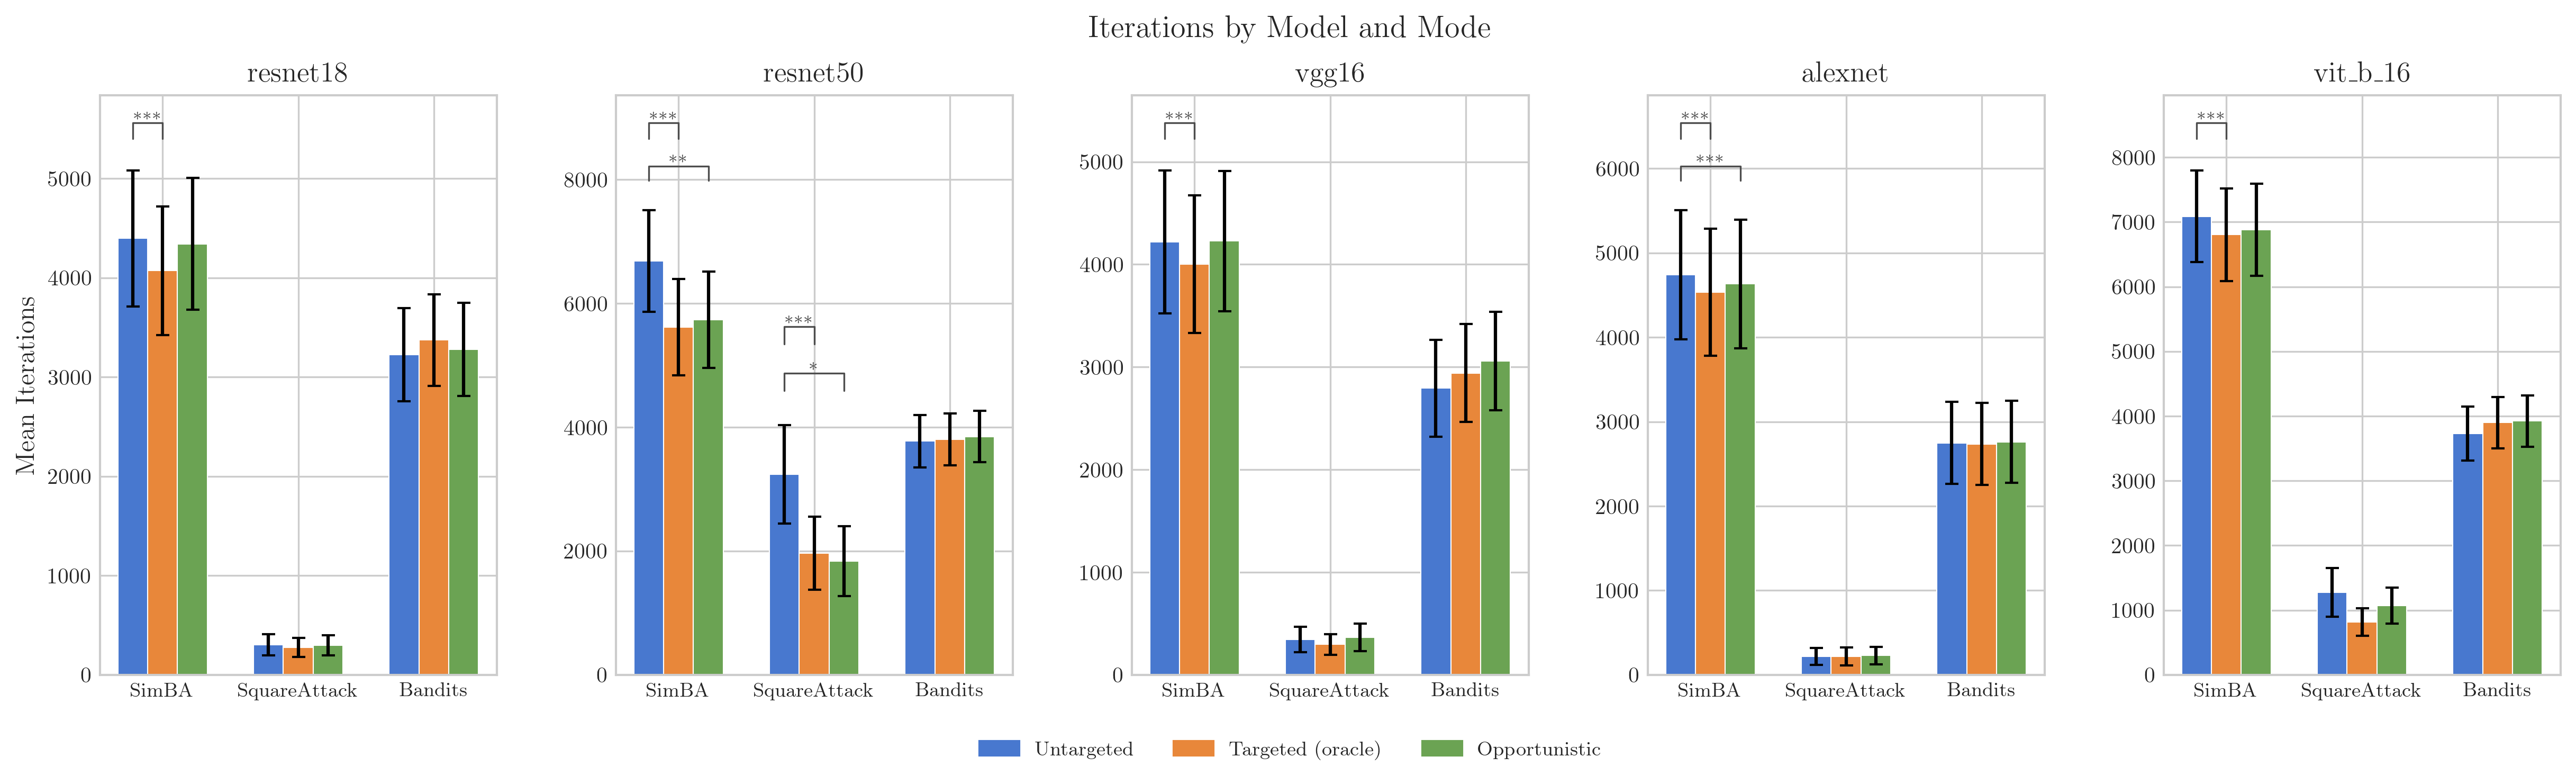
\includegraphics[width=0.85\textwidth]{../results/figures/standard/fig_per_model.png}
\caption{Iterations by model and mode for SimBA, Square Attack (CE), and Bandits. OT's benefit is largest on harder models (ResNet-50, ViT-B/16) and absent for Bandits.}
\label{fig:per-model}
\end{figure*}

\begin{figure*}[t]
\centering
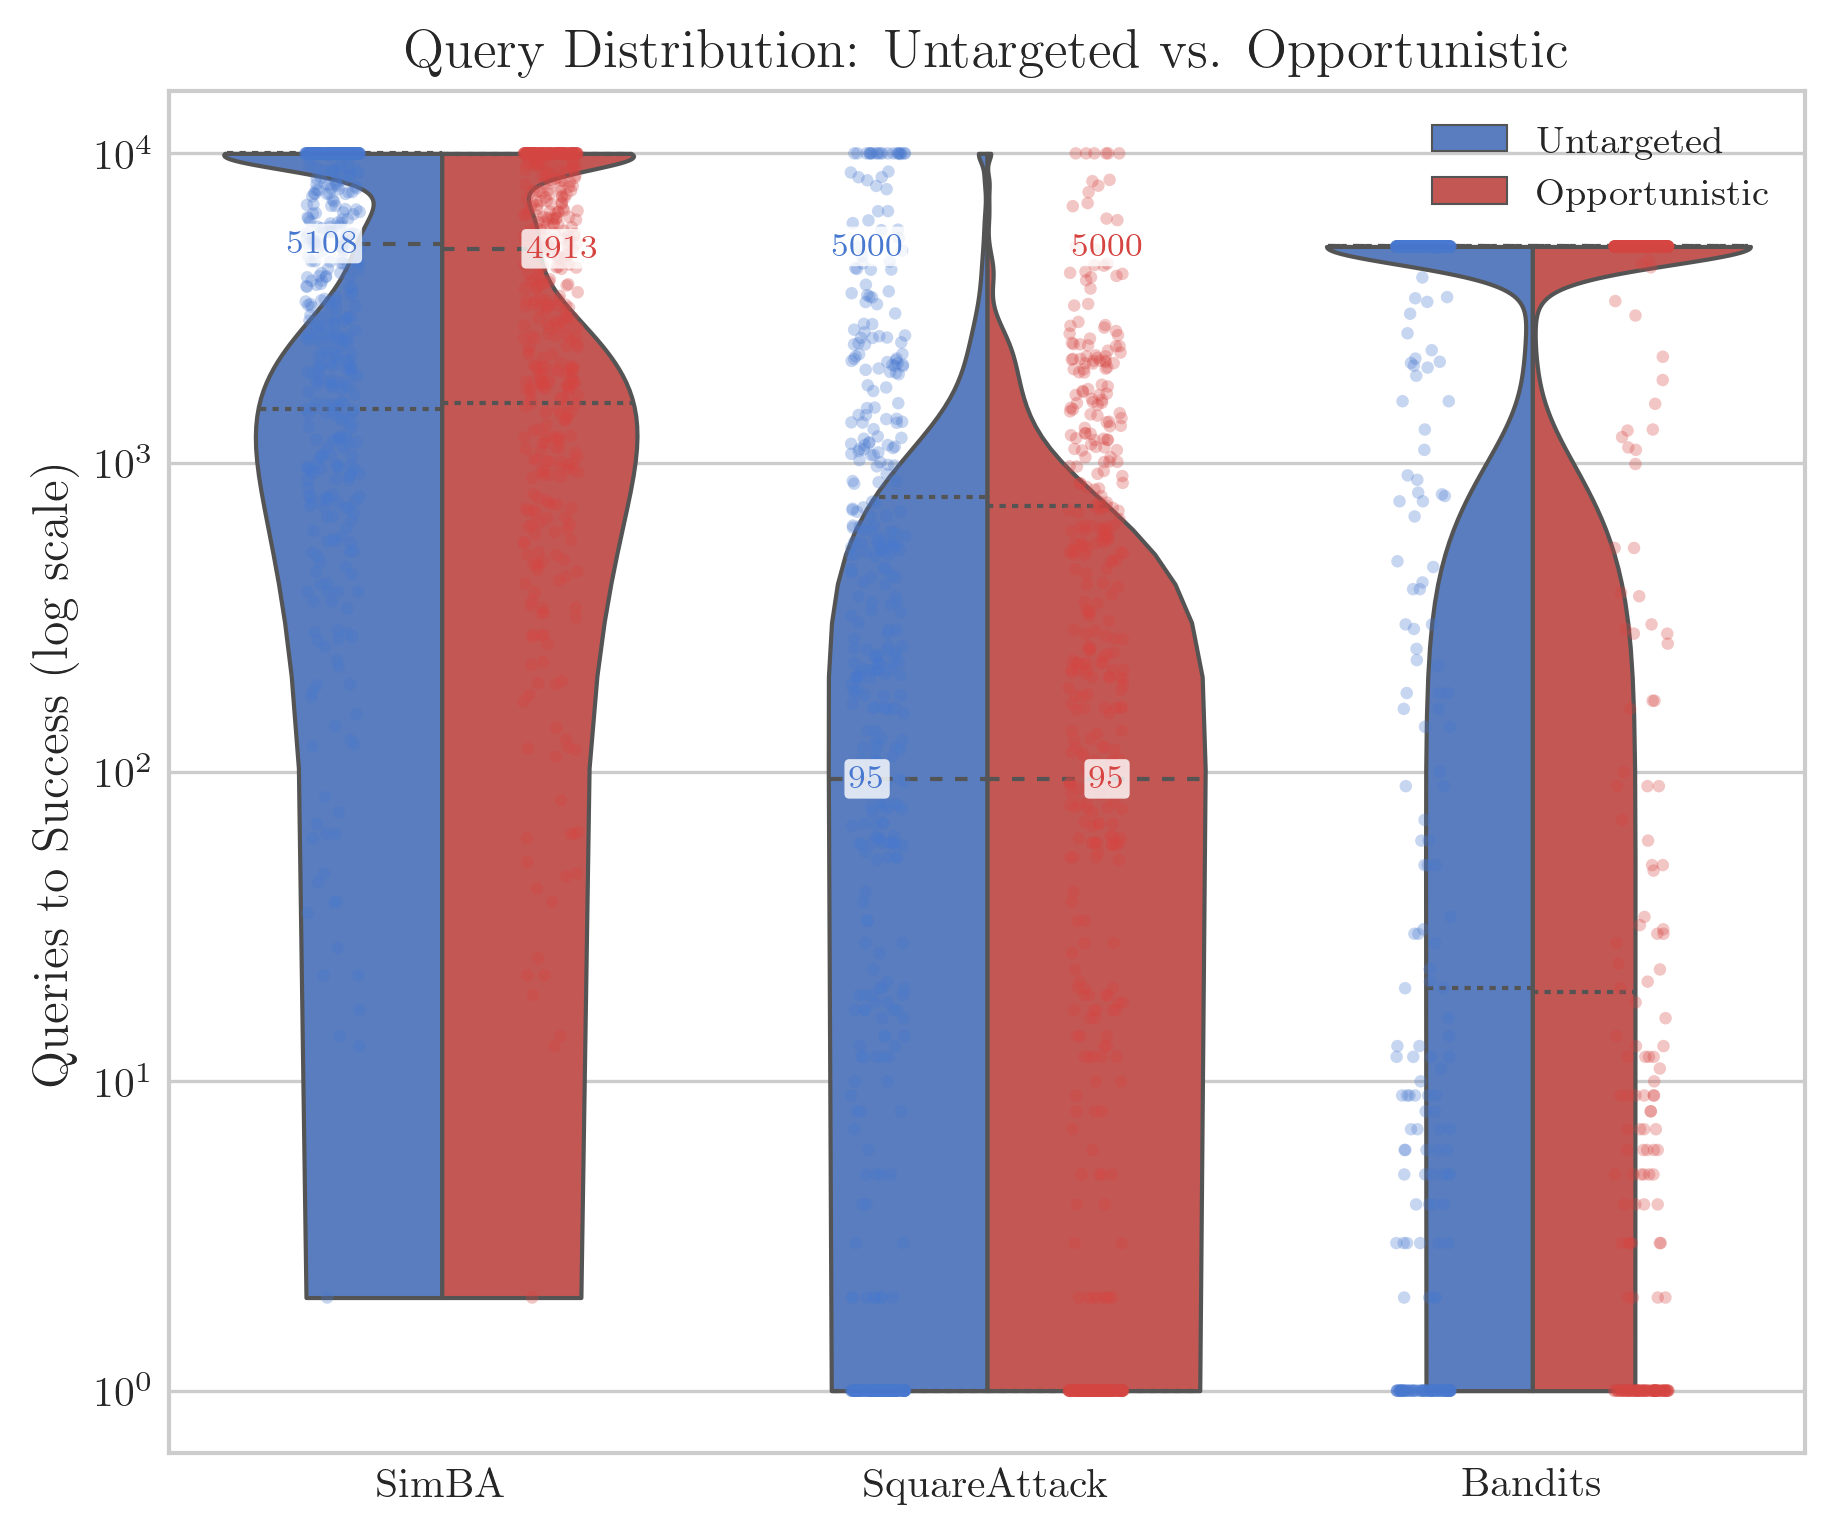
\includegraphics[width=0.85\textwidth]{../results/figures/standard/fig_violin.png}
\caption{Query distribution (log scale). Untargeted (blue) vs.\ Opportunistic (red). Dashed lines show medians.}
\label{fig:violin}
\end{figure*}

\begin{figure*}[t]
\centering
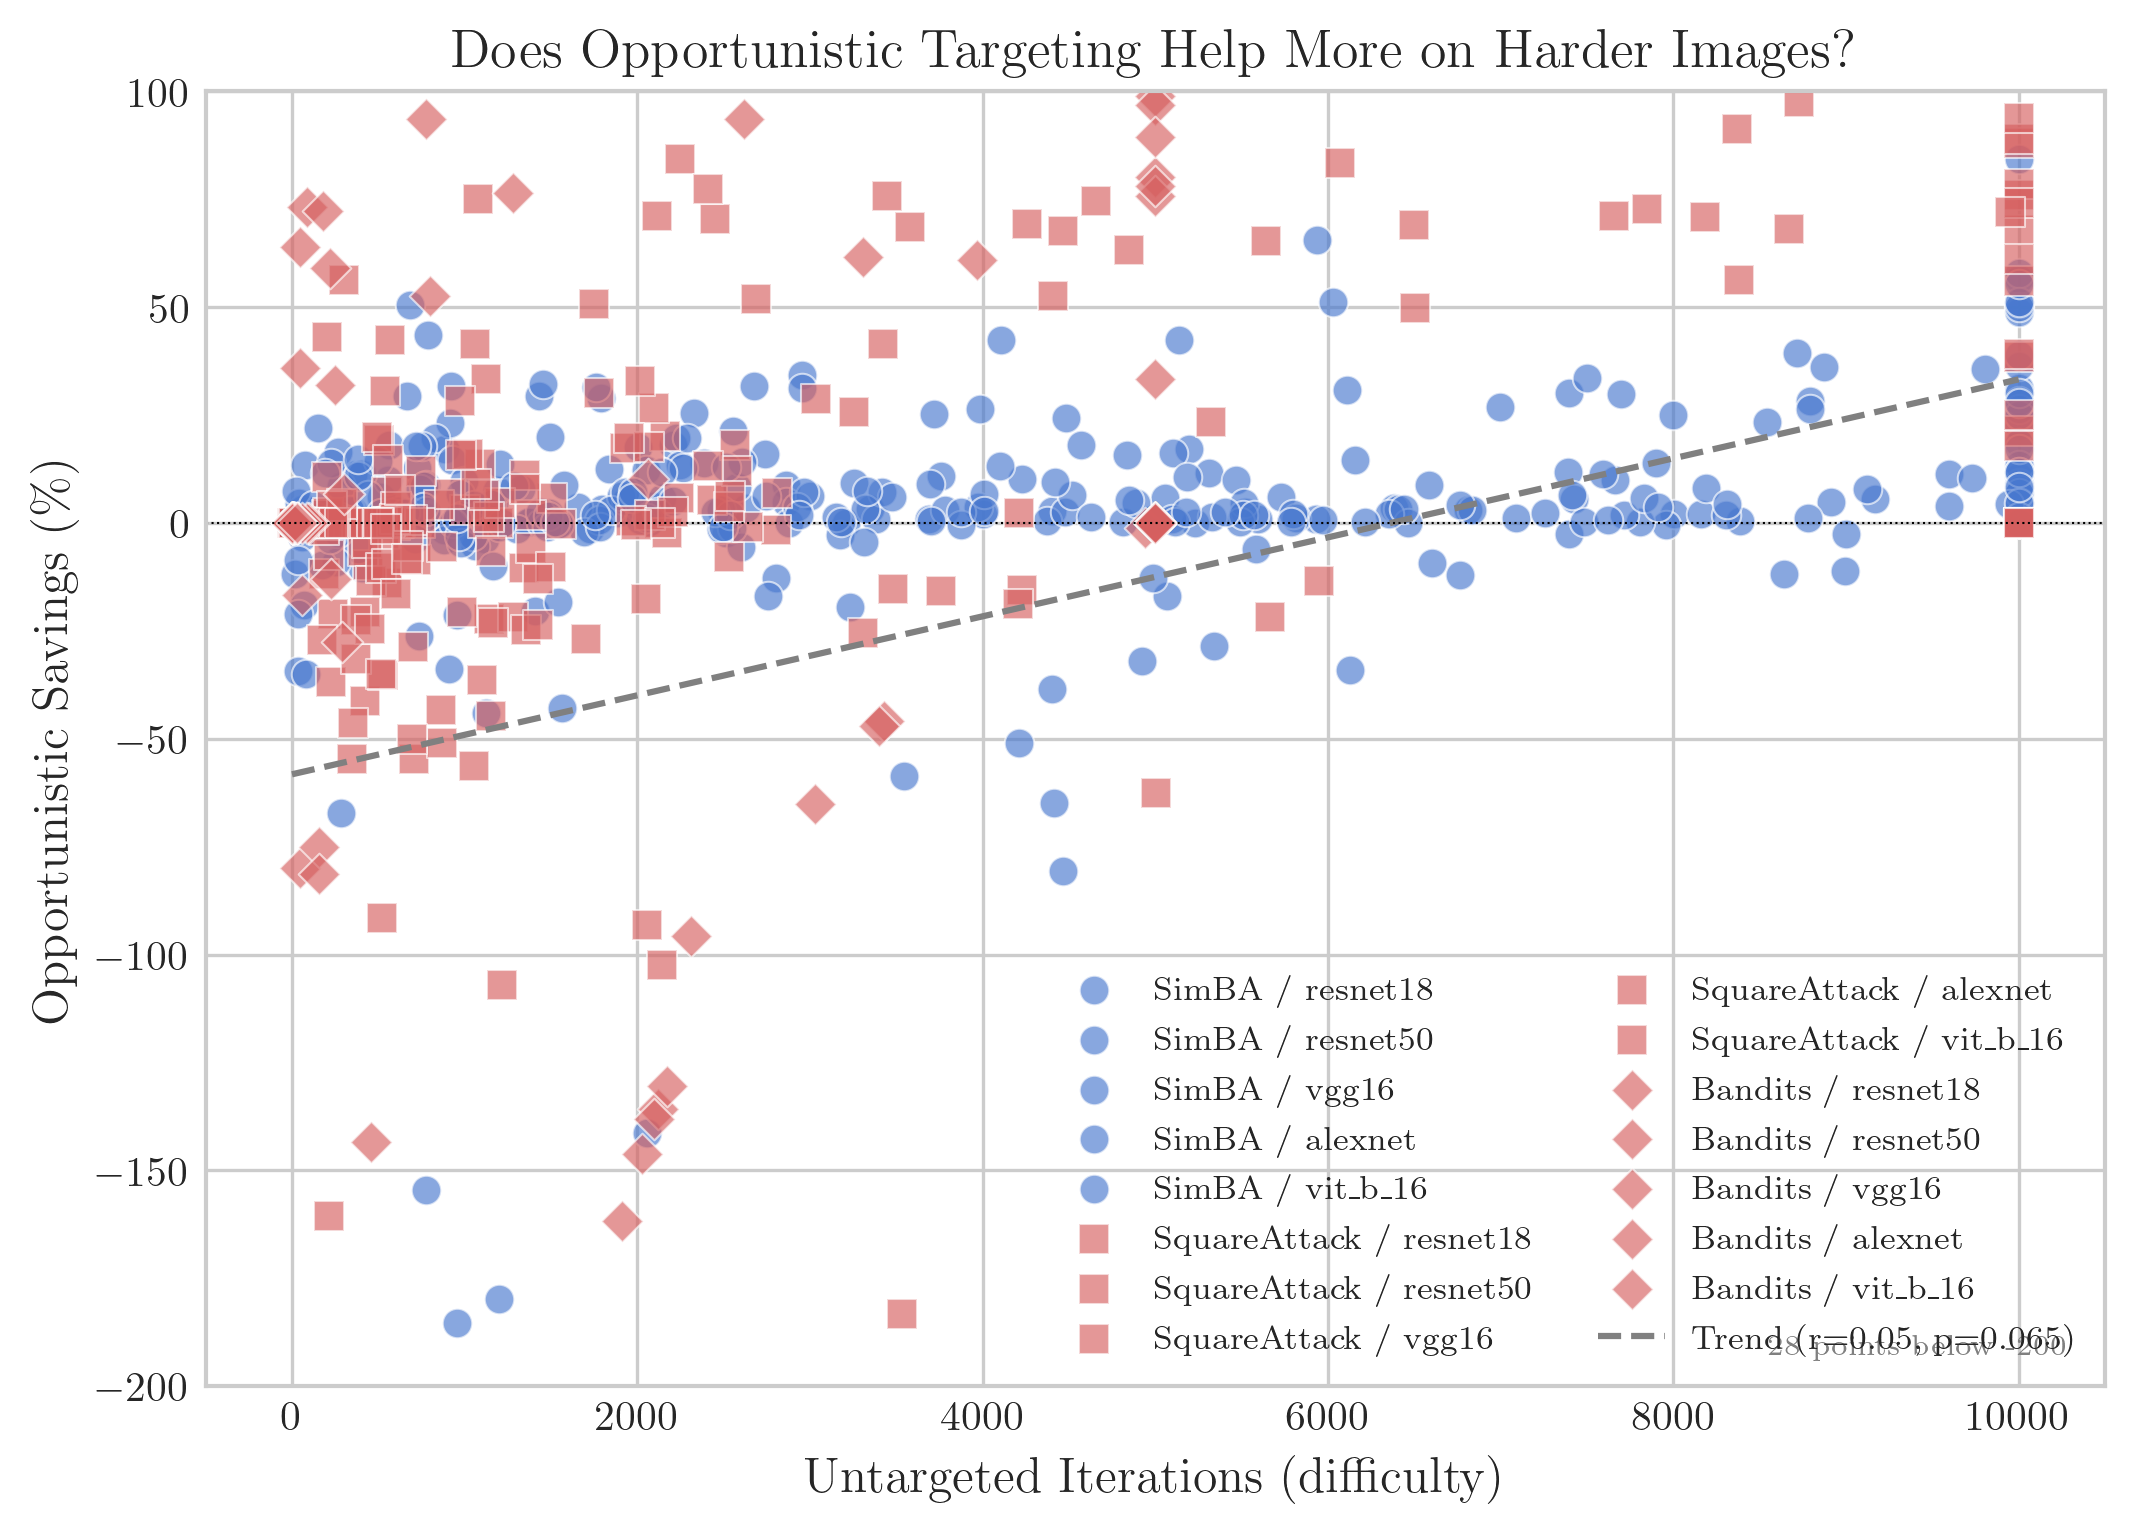
\includegraphics[width=0.85\textwidth]{../results/figures/standard/fig_difficulty_vs_savings.png}
\caption{Opportunistic savings vs.\ attack difficulty. Each point is one (model, method, image) run. Dashed line: linear trend ($r = 0.19$, $p < 0.001$).}
\label{fig:difficulty-savings}
\end{figure*}

\begin{figure*}[t]
\centering
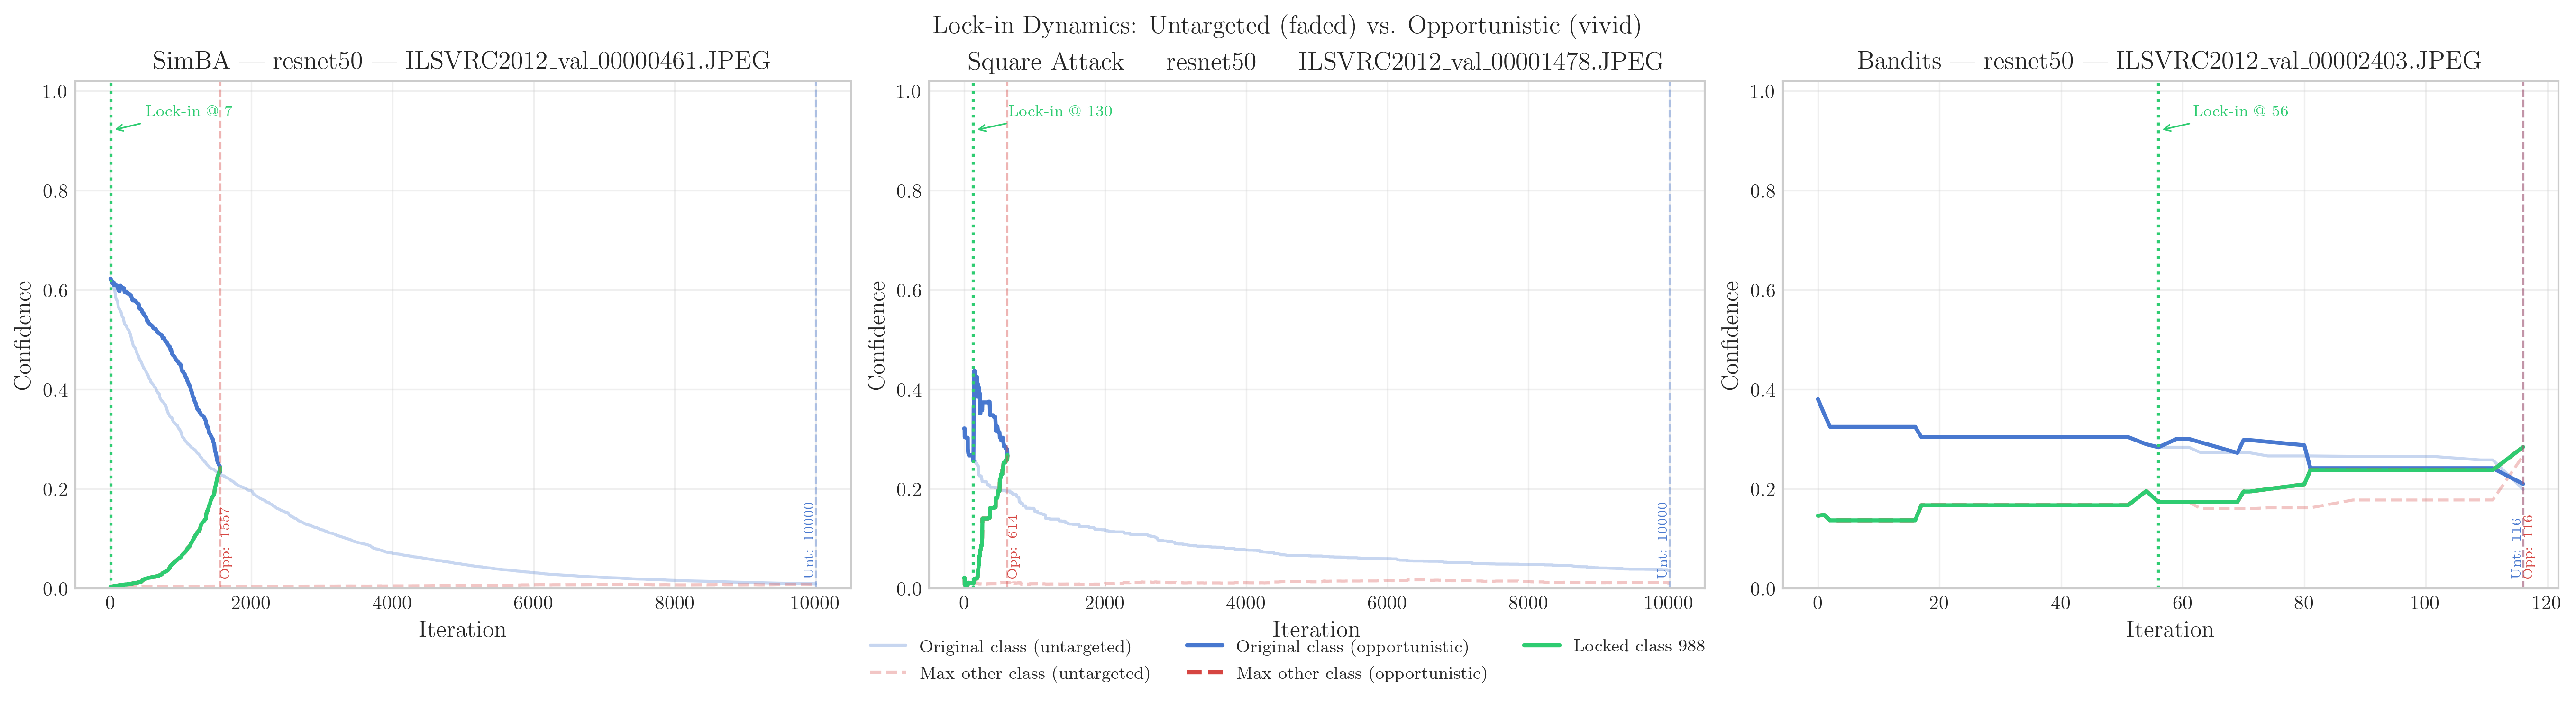
\includegraphics[width=0.85\textwidth]{../results/figures/standard/fig_lockin.png}
\caption{Lock-in dynamics. Faded curves: untargeted; vivid: opportunistic. Vertical dotted lines mark lock-in and convergence iterations. Cases selected as highest-savings image per method from the 50-image benchmark on ResNet-50.}
\label{fig:lockin}
\end{figure*}

\begin{figure*}[t]
\centering
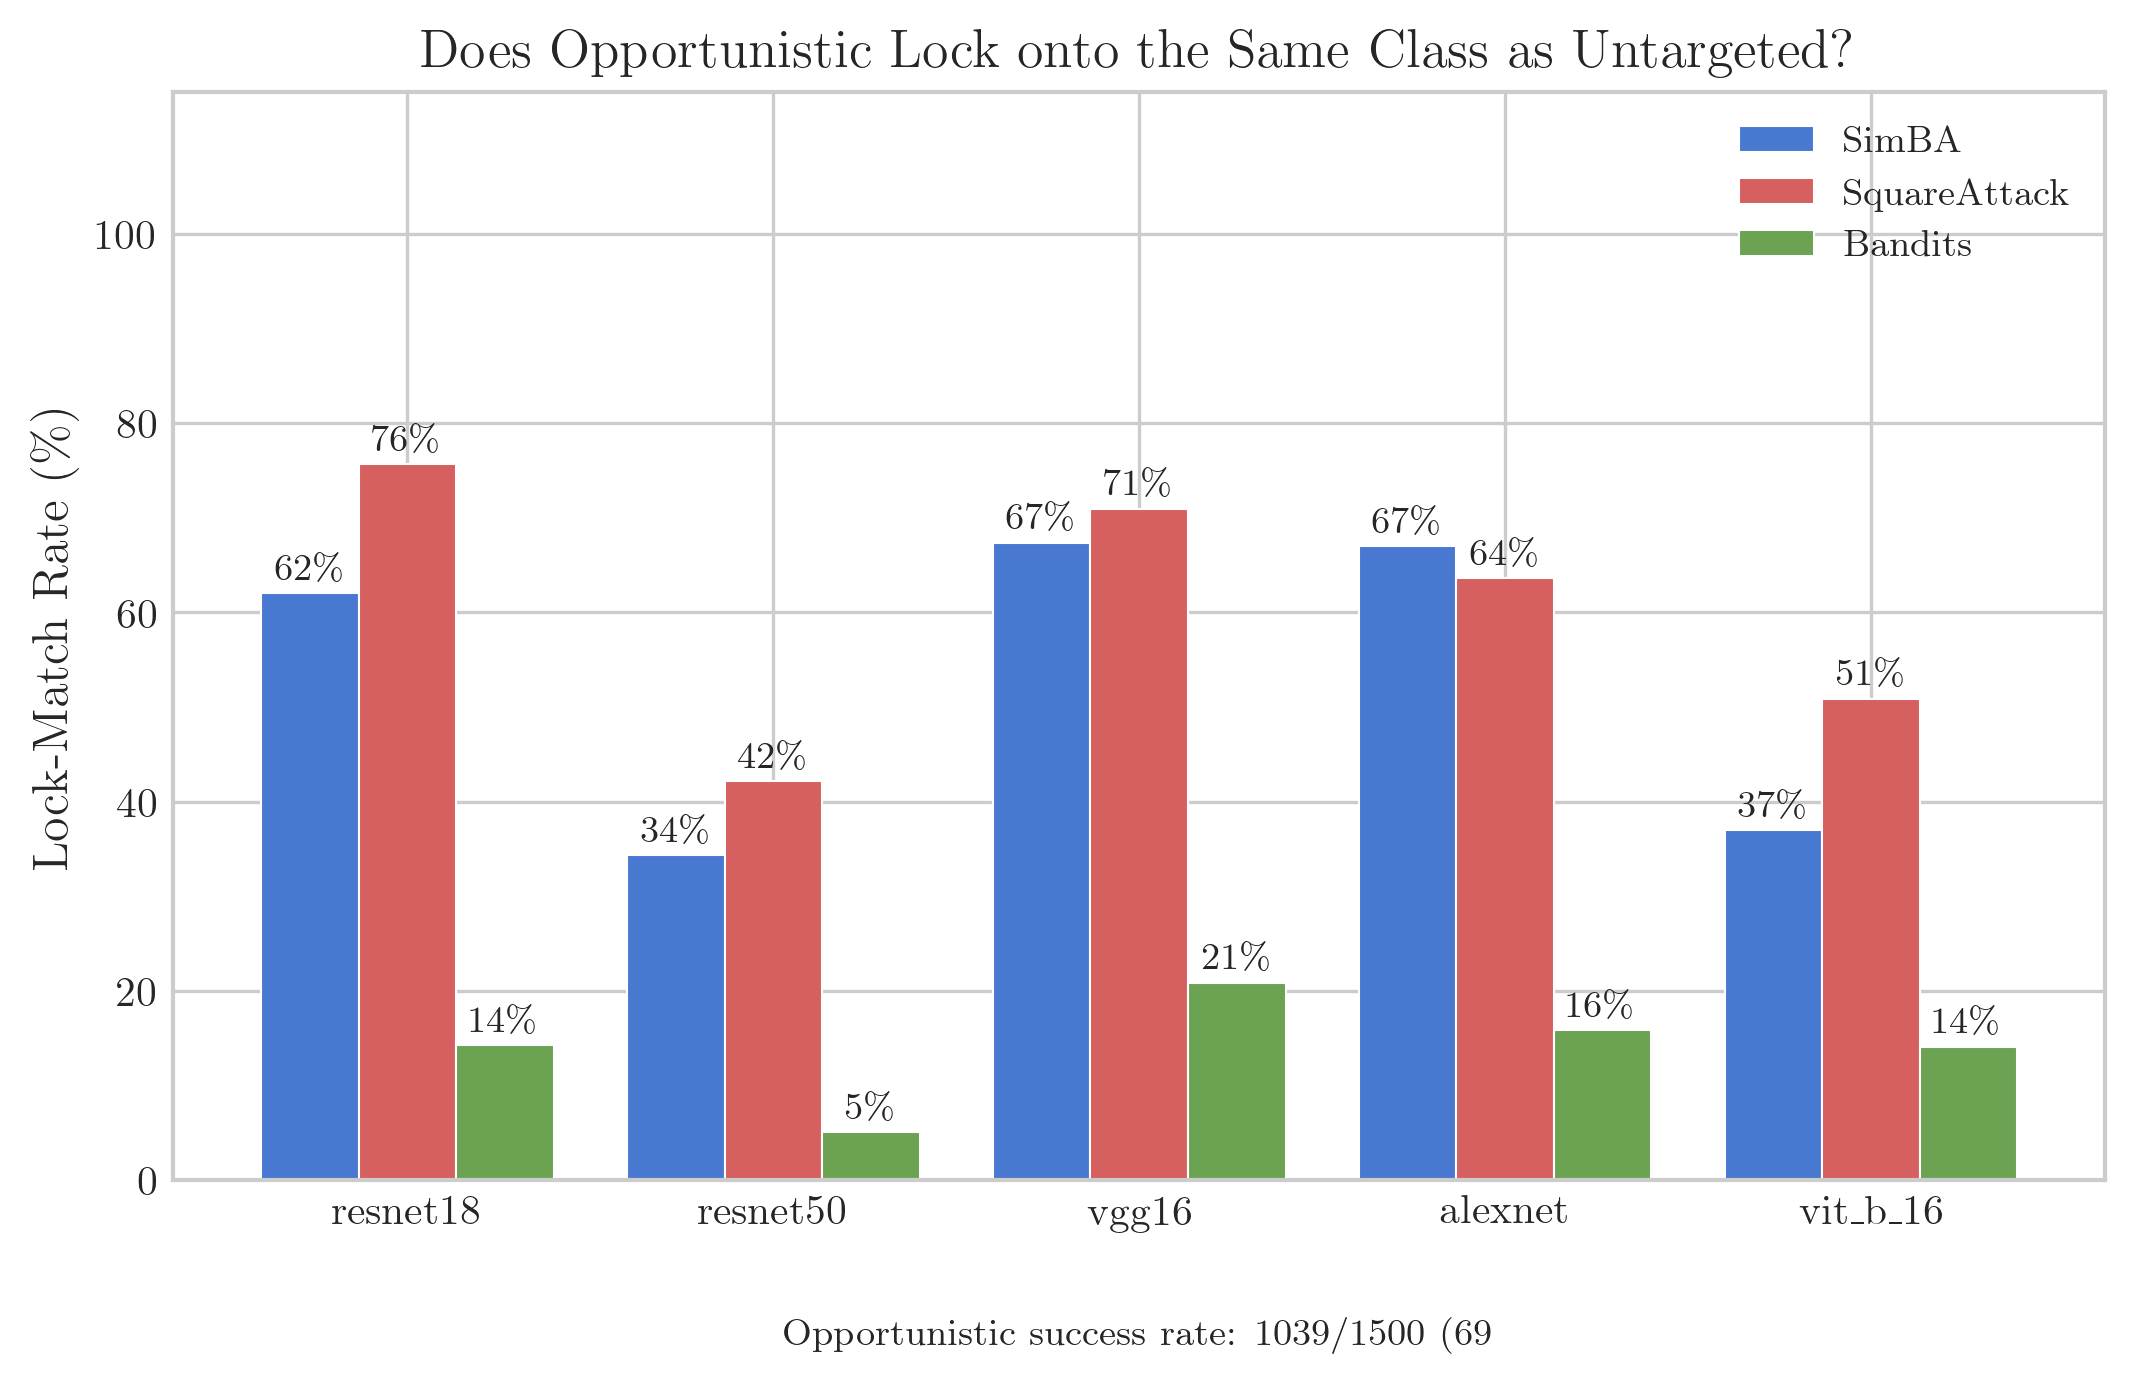
\includegraphics[width=0.85\textwidth]{../results/figures/standard/fig_lock_match.png}
\caption{Lock-match rate by model and method. SimBA and Square Attack show moderate rates (35--75\%). Bandits shows very low rates (5--21\%).}
\label{fig:lock-match}
\end{figure*}

\begin{figure*}[t]
\centering
\includegraphics[width=0.85\textwidth]{../results/figures_lockmatch/fig_lockmatch_correlation.png}
\caption{Per-image savings by lock-match. Left: 50-image benchmark (10K budget), match correlates with savings ($r = 0.31$, $p < 10^{-5}$). Right: 100-image benchmark (15K), correlation vanishes ($r = -0.04$, ns).}
\label{fig:lockmatch-correlation}
\end{figure*}

\section{Ablation Details}\label{app:ablation-details}

\begin{figure*}[t]
\centering
\includegraphics[width=0.85\textwidth]{../results/figures_ablation_s/fig_ablation_s.png}
\caption{Stability threshold ablation. Top: SimBA, bottom: Square Attack (CE). Left: success rate vs.\ $S$; right: mean iterations vs.\ $S$. Dotted lines mark selected $S$.}
\label{fig:s-ablation}
\end{figure*}

\begin{table}[t]
\centering
\caption{SimBA stability threshold sweep (ResNet-50, 100 images, 15K budget).}
\label{tab:simba-s-sweep}
\small
\begin{tabular}{@{}llll@{}}
\toprule
$S$ & Succ.\ Rate & Mean It. & Med.\ It. \\
\midrule
2 & 84.0\% & 4,860 & 4,108 \\
3 & 84.2\% & 4,814 & 3,905 \\
5 & 85.0\% & 4,952 & 4,286 \\
8 & 85.1\% & 4,915 & 4,144 \\
\textbf{10} & \textbf{85.1\%} & \textbf{4,889} & \textbf{4,075} \\
12 & 84.0\% & 4,832 & 4,143 \\
15 & 85.0\% & 4,956 & 4,366 \\
\bottomrule
\end{tabular}
\end{table}

\begin{table}[t]
\centering
\caption{Square Attack stability threshold sweep (ResNet-50, 100 images, 15K budget).}
\label{tab:square-s-sweep}
\small
\begin{tabular}{@{}llll@{}}
\toprule
$S$ & Succ.\ Rate & Mean It. & Med.\ It. \\
\midrule
2 & 97.1\% & 1,917 & 779 \\
3 & 97.1\% & 1,929 & 774 \\
5 & 97.1\% & 2,004 & 754 \\
\textbf{8} & \textbf{98.1\%} & \textbf{1,780} & \textbf{753} \\
10 & 96.1\% & 1,719 & 582 \\
12 & 97.0\% & 1,850 & 633 \\
15 & 96.0\% & 1,910 & 652 \\
\bottomrule
\end{tabular}
\end{table}

\begin{figure*}[t]
\centering
\includegraphics[width=0.85\textwidth]{../results/figures_margin/fig_margin_cdf.png}
\caption{Loss function ablation. Success rate vs.\ query budget for Square Attack on ResNet-50. Margin loss (solid) dominates CE loss (dashed). Margin untargeted alone matches CE + OT, confirming OT as a margin surrogate.}
\label{fig:margin-cdf}
\end{figure*}

\begin{figure*}[t]
\centering
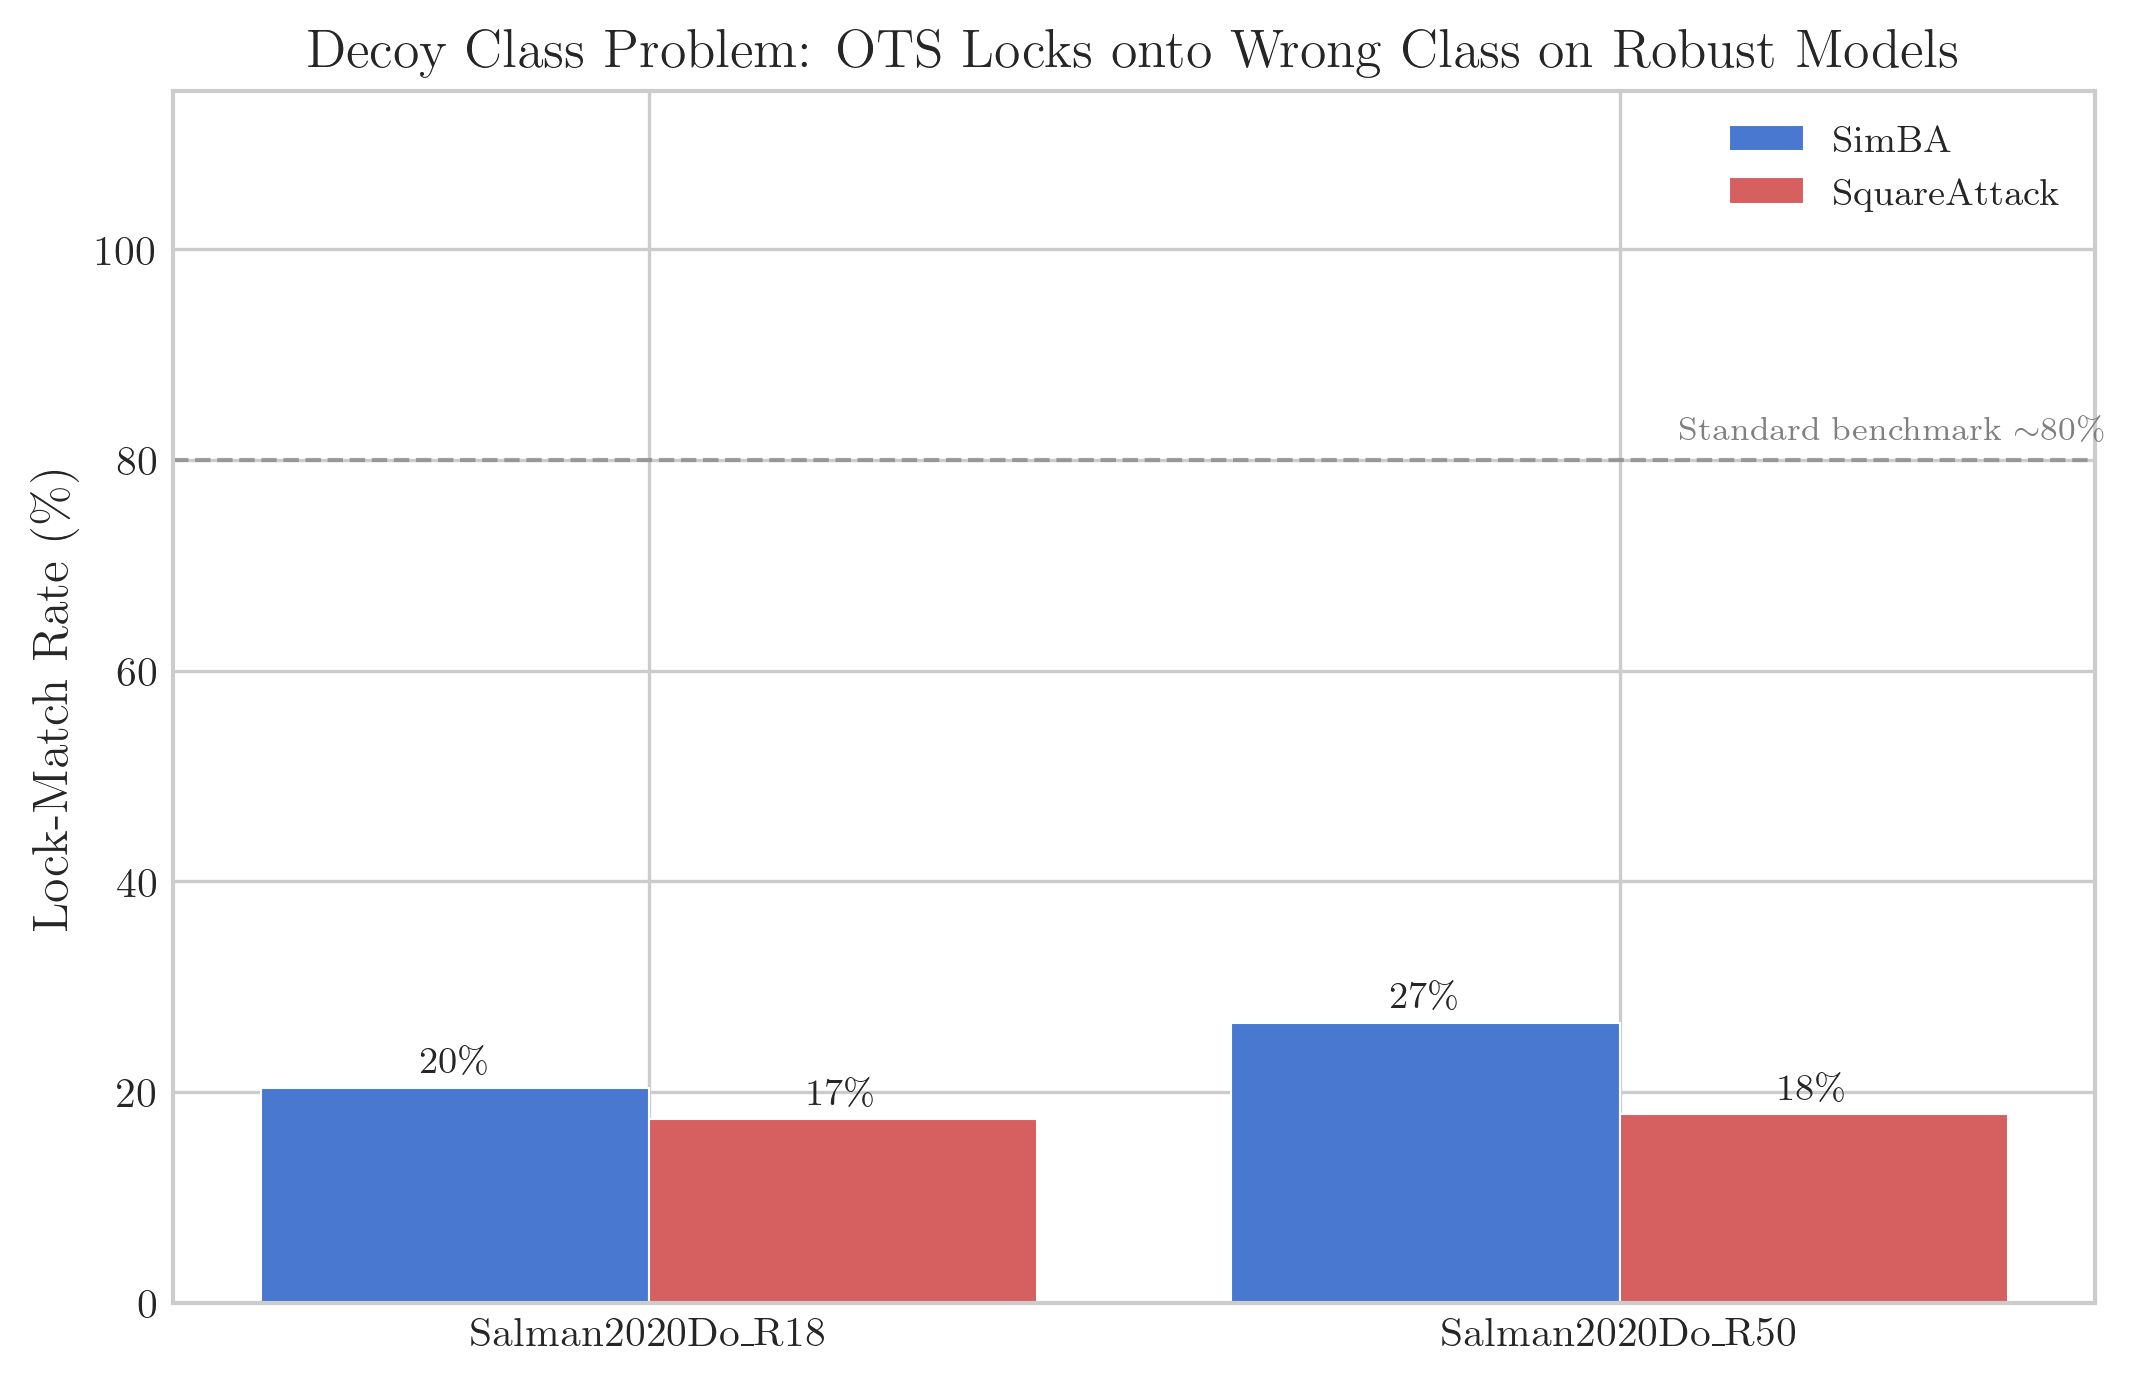
\includegraphics[width=0.85\textwidth]{../results/figures/robust/fig_lock_match.png}
\caption{Lock-match rate on robust models. OT rarely locks the oracle class, reflecting the flatter confidence landscape.}
\label{fig:robust-lock-match}
\end{figure*}

\begin{figure*}[t]
\centering
\includegraphics[width=0.85\textwidth]{../results/figures_ablation_s_robust/fig_ablation_s_robust.png}
\caption{Robust model ablation (Salman2020Do\_R50, 50 images, Square Attack CE). Left: success rate vs.\ $S$. Right: mean iterations vs.\ $S$.}
\label{fig:robust-s-ablation}
\end{figure*}

\end{document}
